\section{Sharp final-support thermal bounds}
\label{sec:bound}

Let $P_L$ be multiplication by $(0,L)$ on $L^2(\R_+)$.  We first solve the
momentum problem at arbitrary inverse temperature $\beta$.  We then impose the
de Sitter relation $\beta=2\pi R$ and prove that the same momentum sector is
the optimum over every angular and canonical sector.

\begin{lemma}[Compressed half-line inverses]
\label{lem:compressed-inverses}
For $h_0=\sqrt{-\partial_x^2}$ with the half-line Dirichlet condition,
\begin{align}
 (P_Lh_0^{-1}P_L)(x,y)
 &=\frac1\pi\log\frac{x+y}{\abs{x-y}},
 \label{eq:hminusone-kernel}\\
 (P_Lh_0^{-2}P_L)(x,y)
 &=\min(x,y).
 \label{eq:hminustwo-kernel}
\end{align}
Moreover,
\begin{align}
 \norm{P_Lh_0^{-1}P_L}
 &\leq \frac{2\operatorname{arsinh}(1)}{\pi}L,
 \label{eq:hminusone-bound}\\
 \norm{P_Lh_0^{-2}P_L}
 &=\frac{4}{\pi^2}L^2.
 \label{eq:hminustwo-bound}
\end{align}
\end{lemma}

\begin{proof}
The unitary sine transform gives
\[
 \frac2\pi\int_0^\infty\frac{\sin(kx)\sin(ky)}{k}\dd k
 =\frac1\pi\log\frac{x+y}{\abs{x-y}}
\]
and
\[
 \frac2\pi\int_0^\infty\frac{\sin(kx)\sin(ky)}{k^2}\dd k
 =\min(x,y).
\]
The logarithmic kernel is positive.  With $u=x/L$, its row integral divided by
$L$ is
\begin{equation}
 \frac1\pi\left[(1+u)\log(1+u)-2u\log u
 -(1-u)\log(1-u)\right].
 \label{eq:row-integral}
\end{equation}
Its maximum is $2\operatorname{arsinh}(1)/\pi$ at $u=1/\sqrt2$, so Schur's
test proves \cref{eq:hminusone-bound}.  The kernel $\min(x,y)$ is the inverse
of $-\partial_x^2$ on $(0,L)$ with Dirichlet condition at zero and Neumann
condition at $L$.  Its first eigenvalue is $(\pi/2L)^2$, proving
\cref{eq:hminustwo-bound}.
\end{proof}

\begin{lemma}[Exact localized KMS kernel]
\label{lem:exact-kms-kernel}
Set
\begin{equation}
 B_{\beta,L}:=P_Lh_0^{-1}\coth(\beta h_0/2)P_L.
\end{equation}
Its integral kernel is
\begin{equation}
 B_{\beta,L}(x,y)
 =\frac1\pi\log\frac{\sinh[\pi(x+y)/\beta]}
 {\sinh[\pi\abs{x-y}/\beta]}.
 \label{eq:exact-kms-kernel}
\end{equation}
Let $\tau=\pi L/\beta$ and define on $L^2(0,1)$
\begin{equation}
 k_\tau(u,v)
 :=\frac1\pi\log\frac{\sinh[\tau(u+v)]}
 {\sinh[\tau\abs{u-v}]},
 \qquad
 \Lambda(\tau):=\norm{\mathcal K_\tau}.
 \label{eq:dimensionless-kernel}
\end{equation}
Then $B_{\beta,L}$ is unitarily equivalent to $L\mathcal K_\tau$.
$\mathcal K_\tau$ is positive, compact, and positivity improving.  Its top
eigenvalue $\Lambda(\tau)$ is simple and has a strictly positive eigenfunction.
\end{lemma}

\begin{proof}
Using $\coth z=1+2\sum_{n\geq1}e^{-2nz}$ and integrating each sine-transform
term gives
\begin{align}
 \frac2\pi\int_0^\infty
 \frac{\sin(kx)\sin(ky)}k\coth(\beta k/2)\dd k
 &=\frac1\pi\log\frac{x+y}{\abs{x-y}}\notag\\
 &\quad+\frac1\pi\sum_{n\geq1}
 \log\frac{(n\beta)^2+(x+y)^2}{(n\beta)^2+(x-y)^2}.
\end{align}
Euler's product for $\sinh$ reduces this expression to
\cref{eq:exact-kms-kernel}.  Scaling $x=Lu$, $y=Lv$ gives the unitary
equivalence.  The logarithmic diagonal singularity is square integrable on the
unit square, so the operator is Hilbert--Schmidt.  The spectral definition
makes it positive, while the displayed kernel is strictly positive away from
the measure-zero boundary and diagonal.  The compact positivity-improving
operator therefore has a simple positive top eigenfunction by the
Perron--Frobenius--Jentzsch theorem.
\end{proof}

\begin{theorem}[Sharp thermal half-line momentum bound]
\label{thm:thermal-half-line}
Let $\beta,L>0$, let $h_0=\sqrt{-\partial_x^2}$ on the Dirichlet half-line,
and define
\begin{equation}
 \mathcal C_\beta(L)
 :=\sup_{\substack{p\neq0\\\supp p\subset[0,L]}}
 \frac{\ip p{h_0^{-1}\coth(\beta h_0/2)p}}{\norm p^2/2}.
 \label{eq:general-cost-definition}
\end{equation}
With $\tau=\pi L/\beta$,
\begin{equation}
 \boxed{\mathcal C_\beta(L)=2L\Lambda(\tau)}.
 \label{eq:general-sharp-cost}
\end{equation}
The normalized optimizer in the finite-energy closure is unique up to sign
and is the positive top eigenfunction of $\mathcal K_\tau$.  The global bounds
\begin{equation}
 \max\left\{\frac{3L}{\pi},\frac{16L^2}{\beta\pi^2}\right\}
 \leq\mathcal C_\beta(L)
 \leq\frac{4\operatorname{arsinh}(1)}\pi L
      +\frac{16L^2}{\beta\pi^2}
 \label{eq:general-explicit-bracket}
\end{equation}
hold for every $\beta,L>0$.  If
\begin{equation}
 M(\tau):=\max_{0<u<1}\int_0^1 k_\tau(u,v)\dd v,
\end{equation}
then $\mathcal C_\beta(L)\leq2LM(\tau)$, and the maximizing row is at
\begin{equation}
 u_\tau=\frac1\tau\operatorname{arsinh}
 \left(\frac{\sinh\tau}{\sqrt2}\right).
 \label{eq:thermal-row-maximizer}
\end{equation}
Finally,
\begin{align}
 0&\leq\mathcal C_\beta(L)-2L\Lambda(0)
 \leq\frac{2\pi L^3}{3\beta^2},
 \label{eq:general-small-support}\\
 0&\leq\mathcal C_\beta(L)-\frac{16L^2}{\beta\pi^2}
 \leq\frac\beta2.
 \label{eq:general-large-support}
\end{align}
Thus the exact answer depends on temperature and support only through
$\tau=\pi L/\beta$, apart from its overall length scale.
\end{theorem}

\begin{proof}
By \cref{lem:exact-kms-kernel}, the quotient in
\cref{eq:general-cost-definition} has supremum
$2\norm{B_{\beta,L}}=2L\Lambda(\tau)$, with the stated unique optimizer.
The profile $p(x)=\sqrt{3/L^3}\,x$ gives the vacuum lower bound $3L/\pi$,
while the first eigenfunction of the Dirichlet--Neumann Green operator and
$\coth z\geq z^{-1}$ give $16L^2/(\beta\pi^2)$.  Conversely,
$\coth z\leq1+z^{-1}$ and \cref{lem:compressed-inverses} give the upper bound
in \cref{eq:general-explicit-bracket}.  Positivity and Schur's test give the
$M(\tau)$ bound.  Differentiating the row integral and using
\begin{equation}
 \sinh[\tau(1+u)]\sinh[\tau(1-u)]
 =\sinh^2\tau-\sinh^2(\tau u)
\end{equation}
gives its unique stationary point \cref{eq:thermal-row-maximizer}.

For small $\tau$, write $k_\tau=k_0+d_\tau$.  Euler's product implies, for
$A\geq B\geq0$,
\begin{equation}
 0\leq\log\frac{\sinh A/A}{\sinh B/B}
 \leq\frac{A^2-B^2}{6}.
\end{equation}
Taking $A=\tau(u+v)$ and $B=\tau\abs{u-v}$ and applying Schur's test gives
$0\leq\Lambda(\tau)-\Lambda(0)\leq\tau^2/(3\pi)$, which proves
\cref{eq:general-small-support}.  For large $\tau$,
\begin{equation}
 k_\tau(u,v)=\frac{2\tau}{\pi}\min(u,v)+r_\tau(u,v).
\end{equation}
The resolvent expansion makes $r_\tau$ nonnegative in operator order, and its
explicit row integral gives $\norm{r_\tau}\leq\pi/(4\tau)$.  Since the norm
of the $\min(u,v)$ operator is $4/\pi^2$, multiplication by $2L$ proves
\cref{eq:general-large-support}.
\end{proof}

The angular potential improves the complete thermal momentum form, not only
the two estimates in \cref{lem:compressed-inverses}.

\begin{lemma}[All-angular and coordinate domination]
\label{lem:angular-domination}
For every $\ell\geq0$, $A_\ell\geq A_0$.  Moreover,
\begin{align}
 h_\ell^{-1}\coth(\beta h_\ell/2)
 &=\frac2\beta A_\ell^{-1}
 +\frac4\beta\sum_{n\geq1}
 \left[A_\ell+(2\pi n/\beta)^2\right]^{-1}
 \notag\\
 &\leq h_0^{-1}\coth(\beta h_0/2)
 \label{eq:thermal-resolvent-order}
\end{align}
as generalized quadratic forms.  If $q$ is supported in $[0,L]$, then
\begin{align}
 \norm q&\leq\frac{L}{\pi}\norm{h_\ell q},
 \label{eq:poincare-q}\\
 \ip q{h_\ell q}
 &\leq\frac{L}{\pi}\norm{h_\ell q}^2,
 \label{eq:fractional-q}\\
 \frac{\Gamma_{q,\ell m}}{E_{q,\ell m}R}
 &\leq\frac{2y}{\pi}+\frac{2y^2}{\pi^3},
 \qquad y=L/R,\qquad \beta=2\pi R.
 \label{eq:coordinate-sector-bound}
\end{align}
\end{lemma}

\begin{proof}
The nonnegative angular potential gives $A_\ell\geq A_0$.  The
Mittag--Leffler expansion $\coth z/z=z^{-2}+2\sum_{n\geq1}
(z^2+\pi^2n^2)^{-1}$ gives \cref{eq:thermal-resolvent-order}; every resolvent
is order decreasing.  Extending $q$ by zero places it in $H_0^1(0,L)$.
Dirichlet Poincare and $\norm{h_\ell q}^2=\ip q{A_\ell q}$ give
\cref{eq:poincare-q}; Cauchy--Schwarz gives \cref{eq:fractional-q}.  Finally,
$\coth z\leq1+z^{-1}$ yields
\begin{equation}
 \Gamma_{q,\ell m}
 \leq\left[\frac L\pi+\frac{2L^2}{\beta\pi^2}\right]
 \norm{h_\ell q}^2.
\end{equation}
Divide by $E_{q,\ell m}=\norm{h_\ell q}^2/2$ and set $\beta=2\pi R$.
No locality of the nonlocal vector $h_\ell q$ is assumed.
\end{proof}

We can now specialize the half-line theorem to the static patch and prove that
no angular or field-coordinate sector gives a larger quotient.  The supremum
below is unchanged if smooth compact data are replaced by their finite-energy
closure.

\begin{theorem}[Conformal de Sitter all-sector optimum]
\label{thm:main}
Let
\begin{equation}
 C_{\rm opt}(y)
 :=\sup\left\{\frac{\Gamma}{\EK R}:
 0<\EK<\infty,\ \supp(q,p)\subset[0,yR]\right\}.
 \label{eq:copt-definition}
\end{equation}
For the full conformally coupled massless scalar in the Bunch--Davies state,
including arbitrary angular data,
\begin{equation}
 \boxed{C_{\rm opt}(y)=2y\Lambda(y/2)}.
 \label{eq:sharp-cost}
\end{equation}
Equivalently,
\begin{equation}
 R C_{\rm opt}(L/R)=\mathcal C_{2\pi R}(L).
 \label{eq:de-sitter-specialization}
\end{equation}
The supremum lies in the s-wave momentum sector.  Its normalized optimizer is
the unique positive top eigenfunction of \cref{eq:dimensionless-kernel}, up to
an overall sign.  Specializing \cref{eq:general-explicit-bracket} gives
\begin{align}
 \max\left\{\frac{3y}{\pi},\frac{8y^2}{\pi^3}\right\}
 &\leq C_{\rm opt}(y)
 \leq F(y),
 \label{eq:global-explicit-bracket}\\
 F(y)&=\frac{4\operatorname{arsinh}(1)}\pi y
 +\frac8{\pi^3}y^2.
 \label{eq:de-sitter-bound}
\end{align}
The sharper bound $C_{\rm opt}(y)\leq2yM(y/2)$ also follows from
\cref{thm:thermal-half-line}.  Its global remainders become
\begin{align}
 0&\leq C_{\rm opt}(y)-2y\Lambda(0)
 \leq\frac{y^3}{6\pi},
 \label{eq:small-support-exact}\\
 0&\leq C_{\rm opt}(y)-\frac{8y^2}{\pi^3}
 \leq\pi.
 \label{eq:large-support-exact}
\end{align}
Thus temperature first corrects the localized vacuum cost at cubic order,
while $8y^2/\pi^3$ is the sharp leading large-support coefficient.
\end{theorem}

\begin{proof}
For momentum data in the s-wave, \cref{thm:thermal-half-line} gives
\begin{equation}
 \sup_{p\neq0}\frac{\Gamma_p}{E_pR}
 =\frac{\mathcal C_{2\pi R}(L)}R
 =2y\Lambda(y/2).
 \label{eq:momentum-optimum}
\end{equation}
Equation~\eqref{eq:thermal-resolvent-order} shows that no higher angular
momentum sector is worse.  The linear trial profile in
\cref{eq:linear-profile} gives the lower bound $3y/\pi$.  Also
$\coth z\geq z^{-1}$ and \cref{eq:hminustwo-bound} give
\begin{equation}
 \sup_{p\neq0}\frac{\Gamma_p}{E_pR}\geq\frac{8y^2}{\pi^3}.
 \label{eq:thermal-lower}
\end{equation}
The right side of \cref{eq:coordinate-sector-bound} is bounded by $3y/\pi$
when $y\leq\pi^2/2$, and by $8y^2/\pi^3$ when $y\geq\pi^2/3$.  These ranges
overlap, so the entire coordinate sector is dominated by the s-wave momentum
supremum for every $y>0$.  The domination is strict for nonzero coordinate
data.  Indeed, at finite $\beta$, the thermal momentum form is strictly larger
than its vacuum part and strictly larger than $(2/\beta)A_0^{-1}$ on every
nonzero vector.  Applying those two strict inequalities to the trial profiles
used above covers the same two overlapping ranges.

The angular domination is also strict for $\ell>0$.  For any $c>0$, the
resolvent difference
$(A_0+c)^{-1}-(A_\ell+c)^{-1}$ has a strictly positive quadratic form on
nonzero data: equality would force
$V_\ell^{1/2}(A_0+c)^{-1}p=0$, where
$V_\ell=\ell(\ell+1)/[R^2\sinh^2(x/R)]>0$ almost everywhere, and hence
$p=0$.  The $n=1$ term of \cref{eq:thermal-resolvent-order} therefore excludes
a higher-angular-momentum tie.  Together with the simple top eigenvalue of
$\mathcal K_{y/2}$, this proves the asserted uniqueness as well as
\cref{eq:sharp-cost}.  The explicit bracket and both remainder bounds are
\cref{eq:general-explicit-bracket,eq:general-small-support} and
\cref{eq:general-large-support} with $\beta=2\pi R$ and $L=yR$.
\end{proof}

\subsection{Numerical realization of the sharp coefficient}

The compact-operator formula can be evaluated directly without entering the
proof.  We use normalized piecewise constants on a uniform partition of
$(0,1)$.  Cell integrals of the vacuum kernel are evaluated exactly from
\begin{equation}
 \frac{\dd^2}{\dd z^2}
 \left(\frac{z^2}{2}\log\abs z-\frac{3z^2}{4}\right)=\log\abs z,
 \label{eq:log-kernel-primitive}
\end{equation}
while Gauss--Legendre quadrature is applied only to the smooth thermal
correction
$\log[\sinh z/z]$.  \Cref{fig:cost-spectrum} shows the resulting
$128$-cell Rayleigh--Ritz curve and positive top eigenfunctions.

At $y=0.1,1,10$ the computed costs are respectively
$0.0997264$, $1.02960$, and $27.7170$.  Across those three points, the largest
relative change from $64$ to $128$ cells is $5.0\times10^{-5}$; changing the
thermal quadrature order from $8$ to $12$ at $64$ cells changes the values by
at most $1.1\times10^{-15}$.  Every one of the nineteen plotted estimates lies
inside \cref{eq:global-explicit-bracket} and below the exact-kernel Schur
bound.  Because the thermal quadrature is not interval enclosed, the plotted
curve is numerical evidence rather than an additional rigorous lower bound;
none of the theorem statements depends on it.

\begin{figure}[tb]
 \centering
 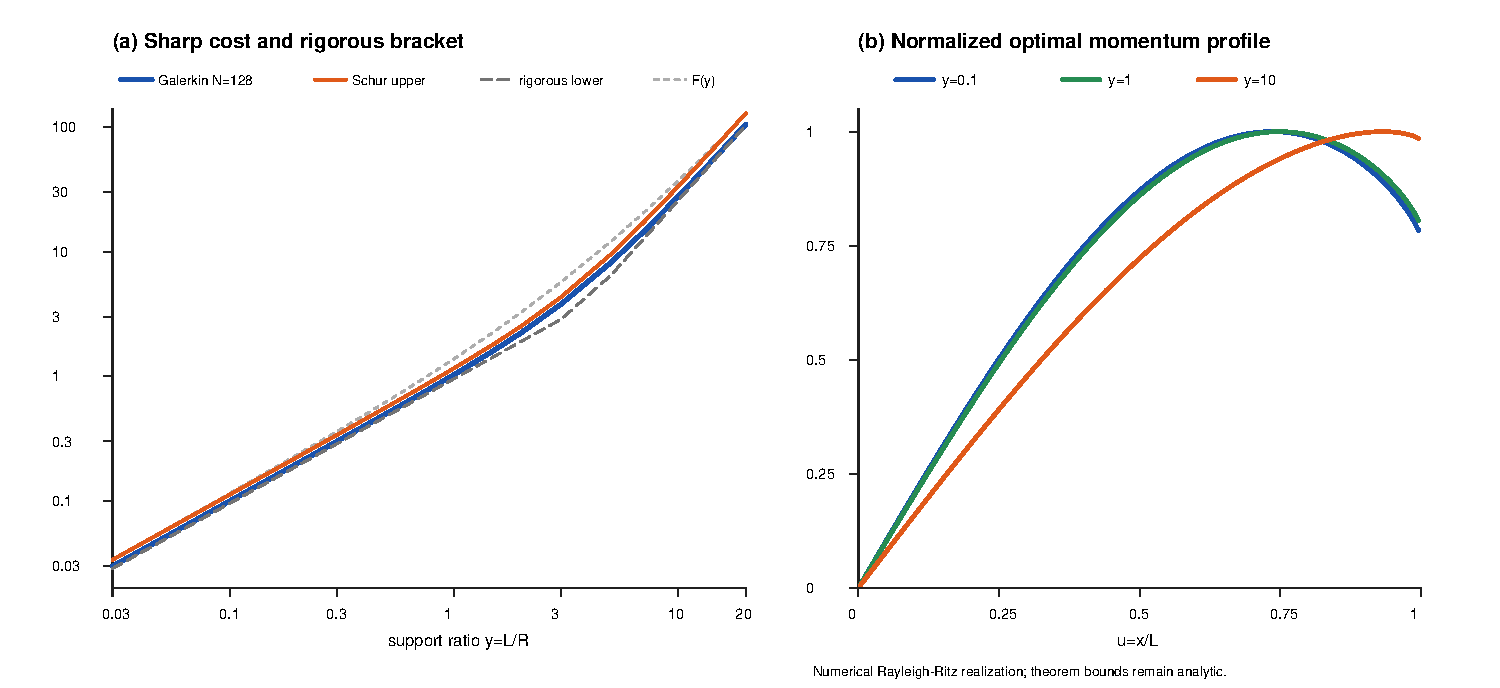
\includegraphics[width=\textwidth]{figures/observer_cost_spectrum.pdf}
 \caption{Numerical realization of the exact compact-kernel theorem.
 Panel (a) compares the $128$-cell Galerkin estimate with the rigorous
 analytic lower bound, the exact-kernel row-Schur upper bound, and the simpler
 closed-form upper bound $F(y)$.  Panel (b) shows the positive top
 eigenfunction, normalized by its maximum, at three support ratios.}
 \label{fig:cost-spectrum}
\end{figure}

Combining \cref{eq:diamond-error,eq:causal-support,eq:sharp-cost} gives the
operational form.

\begin{corollary}[Causal source-cylinder envelope]
\label{cor:source-bound}
If the source in \cref{eq:interaction} is supported in $r\leq a<R$ for a
static-time interval of length $T$, set
\begin{equation}
 y=\operatorname{arctanh}(a/R)+T/R.
\end{equation}
Then
\begin{equation}
 \log\frac{1}{2\eobs}
 \leq \EK R C_{\rm opt}(y)
 =2\EK R y\Lambda(y/2)
 \leq\EK R F(y).
 \label{eq:source-bound}
\end{equation}
The first coefficient is sharp for the relaxed problem in which only the final
Cauchy support $L$ is fixed.  For a cylinder with smaller spatial radius
$\ell=L-T$, the bound remains valid, but reachability of its top eigenfunction
is not asserted.
Exact complete dephasing at finite $a$, $T$, and $R$ requires $\EK=\infty$.
\end{corollary}

\begin{remark}
The final statement is a no-go only for exact complete dephasing in the frozen
local scalar model.  It is not a universal energy cost for quantum
measurement, and it does not price the external device used to realize $J$.
\end{remark}
